\chapter{Application Text-to-SQL avec Cortex AI}
\label{ch:application}

\section{Choix du service : Cortex Analyst}

Deux approches étaient envisageables pour générer le SQL avec Snowflake Cortex :
\begin{enumerate}
  \item appeler une fonction LLM générique (\texttt{SNOWFLAKE.CORTEX.COMPLETE}) en lui fournissant la
        question et une description textuelle du schéma ;
  \item utiliser \textbf{Cortex Analyst}, service spécialisé guidé par un modèle sémantique.
\end{enumerate}

Les tests réalisés sur le compte ont tranché la question : sur un \textbf{compte d'essai} Snowflake,
toutes les fonctions LLM génériques (\texttt{COMPLETE}, \texttt{AI\_COMPLETE}, \texttt{SENTIMENT},
\texttt{AI\_CLASSIFY}\ldots) sont désactivées et renvoient l'erreur
« \emph{AI function \ldots{} is not available for trial accounts} ». Cortex Analyst, en revanche, est
disponible. Ce choix est par ailleurs le plus pertinent techniquement : le modèle sémantique encode la
connaissance métier (synonymes, calculs, jointures) et produit un SQL nettement plus fiable qu'une
génération libre.

\section{Le modèle sémantique}

Le fichier \texttt{app/semantic\_model.yaml} décrit la couche Gold pour Cortex Analyst :
\begin{itemize}
  \item \textbf{10 tables logiques} (5 faits, 5 dimensions), chacune avec ses dimensions, dimensions
        temporelles, faits et métriques ;
  \item \textbf{des synonymes français} : « CA », « chiffre d'affaires », « ventes » pour
        \texttt{amount\_excluding\_tax} ; « marge », « bénéfice » pour \texttt{profit} ;
        « commercial », « vendeur » pour \texttt{employee\_name}\ldots ;
  \item \textbf{des valeurs d'exemple} (\texttt{sample\_values}) relevées dans les données réelles, qui
        aident le modèle à traduire « supermarchés » en \texttt{'Supermarket'} ;
  \item \textbf{des métriques} : chiffre d'affaires total, bénéfice total, taux de marge, nombre de
        factures et de commandes ;
  \item \textbf{11 relations} de type plusieurs-à-un entre faits et dimensions ;
  \item \textbf{3 requêtes vérifiées} correspondant aux questions de l'énoncé ;
  \item \textbf{des instructions personnalisées} : répondre en français, considérer par défaut le CA hors
        taxes, limiter les classements à 10 lignes, arrondir à deux décimales.
\end{itemize}

\begin{lstlisting}[language=yaml, caption={Extrait du modèle sémantique : table des ventes et métrique de marge}, label=lst:semantic]
- name: fact_sales
  description: Ventes facturées, une ligne par ligne de facture.
  base_table: {database: WWI_DB, schema: GOLD, table: FACT_SALES}
  primary_key: {columns: [invoice_line_id]}
  time_dimensions:
    - {name: invoice_date, expr: invoice_date, data_type: date,
       synonyms: [date de vente, date de facture, date]}
  facts:
    - {name: amount_excluding_tax, expr: amount_excluding_tax, data_type: number,
       synonyms: [chiffre d'affaires, CA, ventes, revenu, montant HT]}
    - {name: profit, expr: profit, data_type: number, synonyms: [bénéfice, marge, profit]}
  metrics:
    - {name: margin_rate, expr: "SUM(profit) / NULLIF(SUM(amount_excluding_tax), 0)",
       description: Taux de marge (bénéfice / CA HT), synonyms: [taux de marge]}
\end{lstlisting}

\begin{infobox}[title=Point d'attention rencontré]
Dans la syntaxe YAML compacte \texttt{\{clé: valeur, \ldots\}}, une virgule non protégée termine la
valeur. L'expression \texttt{NULLIF(SUM(\ldots), 0)} était ainsi tronquée et Cortex Analyst rejetait le
modèle (« \emph{Invalid semantic model yaml} »). Toute expression contenant une virgule doit être placée
entre guillemets.
\end{infobox}

\section{Fonctionnement de l'application}

La figure~\ref{fig:sequence} décrit le traitement d'une question.

\begin{figure}[H]
\centering
\resizebox{\linewidth}{!}{%
\begin{tikzpicture}[
  actor/.style={draw, rounded corners=3pt, fill=ucadblue!12, font=\footnotesize\bfseries, minimum width=2.6cm, minimum height=0.8cm},
  msg/.style={-{Stealth[length=2.2mm]}, thick},
  ret/.style={-{Stealth[length=2.2mm]}, thick, dashed},
  note/.style={font=\scriptsize, fill=white, inner sep=1.5pt}]
  \node[actor] (u) at (0,0) {Décideur};
  \node[actor] (st) at (4.2,0) {Streamlit};
  \node[actor, fill=snow!20] (ca) at (8.8,0) {Cortex Analyst};
  \node[actor, fill=gold!30] (g) at (13.2,0) {Snowflake GOLD};
  \foreach \n in {u,st,ca,g} \draw[black!30] (\n.south) -- ++(0,-6.4);
  \draw[msg] (0,-0.9) -- node[note, above]{« Quels produits génèrent le plus de bénéfices ? »} (4.2,-0.9);
  \draw[msg] (4.2,-1.7) -- node[note, above]{question + historique + modèle sémantique} (8.8,-1.7);
  \draw[ret] (8.8,-2.5) -- node[note, above]{interprétation + requête SQL} (4.2,-2.5);
  \draw[msg] (4.2,-3.1) -- ++(0.9,0) |- node[note, right, pos=0.25]{contrôle lecture seule} (4.25,-3.7);
  \draw[msg] (4.2,-4.4) -- node[note, above]{exécution (rôle \texttt{WWI\_ANALYST})} (13.2,-4.4);
  \draw[ret] (13.2,-5.2) -- node[note, above]{résultats} (4.2,-5.2);
  \draw[ret] (4.2,-6.0) -- node[note, above]{interprétation, SQL, graphique, tableau, CSV} (0,-6.0);
\end{tikzpicture}}
\caption{Traitement d'une question en langage naturel}
\label{fig:sequence}
\end{figure}

\subsection{Architecture du code}
Le code est séparé en deux modules :
\begin{itemize}
  \item \texttt{cortex\_analyst.py} : le \emph{moteur}, indépendant de l'interface. Il envoie la
        conversation à Cortex Analyst, contrôle et exécute le SQL. Il propose deux implémentations
        interchangeables : \texttt{LocalBackend} (connecteur Python et identifiants du fichier
        \texttt{.env}) et \texttt{SnowflakeBackend} (session active de Streamlit in Snowflake, sans
        identifiant à gérer) ;
  \item \texttt{streamlit\_app.py} : l'\emph{interface} de conversation.
\end{itemize}

\subsection{Conversation multi-tours}
L'historique complet des échanges est transmis à Cortex Analyst à chaque question. Les questions de
suivi sont ainsi interprétées dans leur contexte : après « Quel est le chiffre d'affaires par catégorie
de client et par année ? », la question « Et seulement pour les supermarchés, par mois en 2015 ? » est
correctement comprise comme « \emph{le chiffre d'affaires HT par mois en 2015, uniquement pour la
catégorie de client Supermarket} ».

\subsection{Choix automatique de la visualisation}
L'application analyse le résultat pour choisir la représentation la plus adaptée :
\begin{itemize}
  \item une valeur unique est affichée comme un \textbf{indicateur} (KPI) ;
  \item si une colonne est temporelle (date, mois, année\ldots), une \textbf{courbe} est tracée, avec une
        série par catégorie si une seconde dimension est présente ;
  \item sinon, un \textbf{diagramme en barres} horizontal trié par valeur décroissante est affiché.
\end{itemize}
Les colonnes numériques représentant le temps (année, mois) ou des identifiants sont traitées comme des
axes et non comme des mesures.

\section{Sécurité de la génération de SQL}

Confier l'écriture du SQL à un modèle de langage impose des garde-fous. Trois niveaux de protection se
cumulent :
\begin{enumerate}
  \item \textbf{Contrôle syntaxique} avant exécution (listing~\ref{lst:guard}) : une seule instruction,
        commençant par \texttt{SELECT} ou \texttt{WITH}, sans aucun mot-clé d'écriture ou
        d'administration ;
  \item \textbf{Moindre privilège} : la requête est exécutée avec le rôle \texttt{WWI\_ANALYST}, qui ne
        peut que lire le schéma Gold ;
  \item \textbf{Limitation des volumes} : 10\,000 lignes au maximum sont rapatriées.
\end{enumerate}

\begin{lstlisting}[language=Python, caption={Contrôle de lecture seule du SQL généré}, label=lst:guard]
FORBIDDEN = re.compile(
    r"\b(insert|update|delete|merge|drop|create|alter|truncate|grant|revoke"
    r"|call|copy|put|remove|use|execute)\b", re.IGNORECASE)

def check_read_only(sql: str) -> None:
    """Refuse toute requête qui n'est pas une simple lecture."""
    stripped = re.sub(r"--[^\n]*|/\*.*?\*/", "", sql, flags=re.DOTALL).strip().rstrip(";")
    if ";" in stripped:
        raise ValueError("Une seule instruction SQL est autorisée.")
    if not re.match(r"^(with|select)\b", stripped, re.IGNORECASE):
        raise ValueError("Seules les requêtes SELECT sont autorisées.")
    if FORBIDDEN.search(stripped):
        raise ValueError("La requête contient une instruction non autorisée.")
\end{lstlisting}

\section{Interface utilisateur}

L'interface reprend l'identité visuelle de l'Université Cheikh Anta Diop : un en-tête présente le logo,
le nom de l'université et de la faculté, et un pied de page rappelle le département, la section et la
formation. La barre latérale propose des questions d'exemple et la réinitialisation de la conversation.

\begin{figure}[H]
\centering

\includegraphics[width=0.88\linewidth]{figures/app_accueil.jpg}
\caption{Page d'accueil de l'application : en-tête UCAD, exemples de questions et pied de page}
\label{fig:app-accueil}
\end{figure}

\begin{figure}[H]
\centering
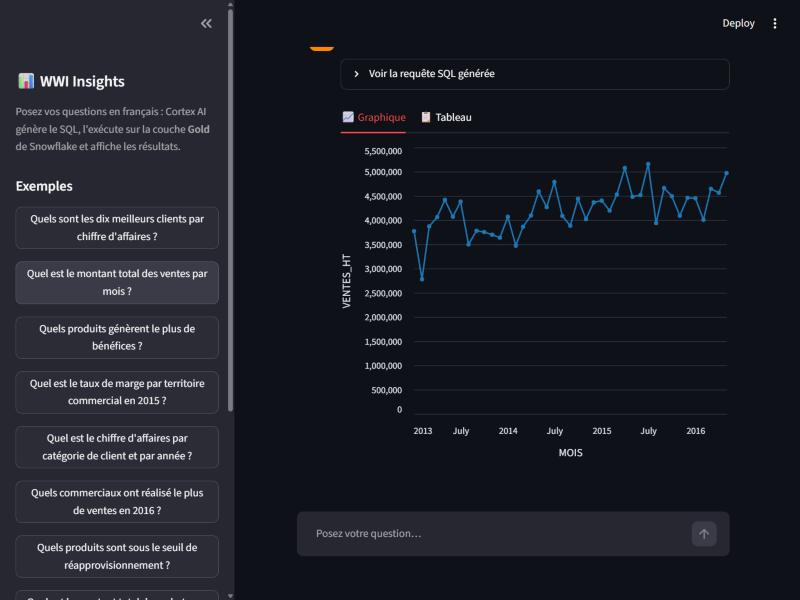
\includegraphics[width=0.88\linewidth]{figures/app_ventes_mois.jpg}
\caption{« Quel est le montant total des ventes par mois ? » : courbe générée automatiquement}
\label{fig:app-mois}
\end{figure}

\begin{figure}[H]
\centering
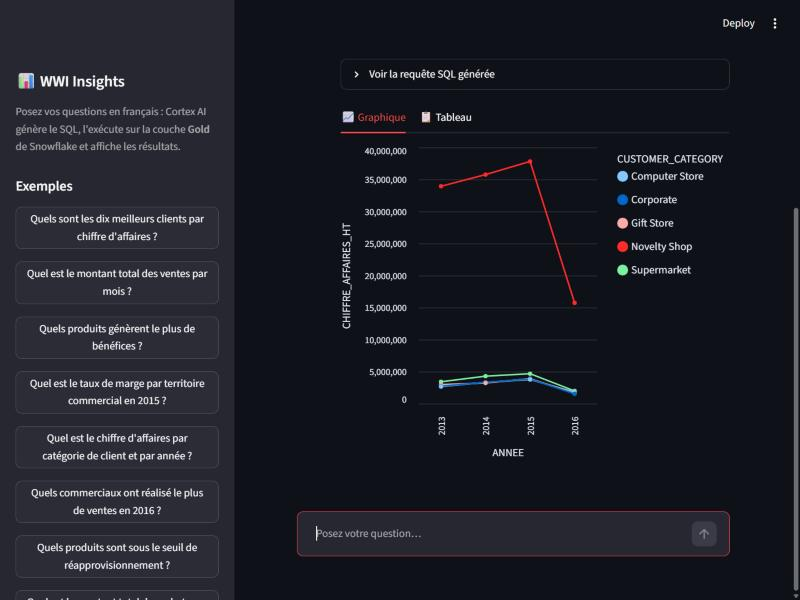
\includegraphics[width=0.88\linewidth]{figures/app_categorie_annee.jpg}
\caption{« Quel est le chiffre d'affaires par catégorie de client et par année ? » : une série par catégorie}
\label{fig:app-categorie}
\end{figure}

Pour chaque réponse, l'utilisateur dispose de l'interprétation de sa question par Cortex Analyst, de la
requête SQL générée (dans un panneau dépliable, pour la transparence et l'apprentissage), du graphique,
du tableau de résultats et d'un export CSV. En cas d'ambiguïté, Cortex Analyst propose des
reformulations cliquables.
